\documentclass[a4paper,12pt]{article}

\usepackage[margin=1in]{geometry}
\usepackage{tikz}
\usepackage{amssymb}
\usepackage{xcolor}
\usepackage{circuitikz}
\usepackage{graphicx}

\newcommand{\ra}{$\rightarrow$}
\newenvironment{6mini}{
  \begin{minipage}{6cm}
}{
  \end{minipage}
}

\title{\texttt{Frequency Division}\\\hrulefill}
\author{Module 16}
\date{\small{11/25/2023}}

\begin{document}
    \maketitle

    \section{Cascading Counters}
        Cascading a counter effectively makes a larger counter/ increases the MOD of the counter. MOD will determine frequency division, thus having a higher MOD prompts the need of cascading counters.
        \begin{itemize}
            \item The effective MOD of the cascaded counter is the product of all the MODs of each other
            \item MOD 4 counter cascaded with a MOD 8 will result in a MOD 32 counter.
        \end{itemize}
        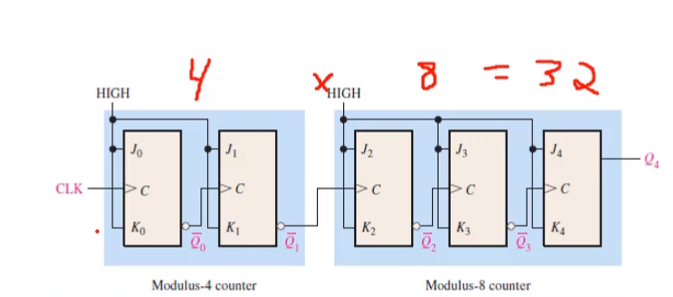
\includegraphics[width=12cm]{CASMOD1.png}\\Cascading asynchronous counters
           \subsection{4 bit Synchronous counter}
            Cascading synchronous counters require some additional inputs.
            \begin{itemize}
                \item A. B, C, D are initial values to load into the counter \ra~use if the ocunter starts at a specific value (A is LSB)
                \item load will place the inital value set by A, B, C, and D inputs into the ocunter onthe next clock edge.
                \item Clear resets the counter to 0000
                \item ENP and ENT are enables, both must be HIGH for the ocunter to work. ENP enables the clock, ENT enables the terminal count (acknowlege when 1111 is reached).
            \end{itemize}
            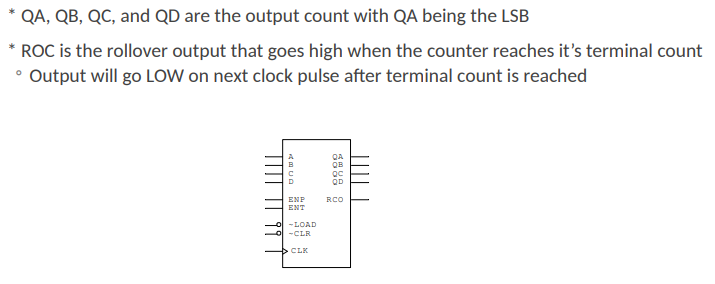
\includegraphics[width=15cm]{4bitsyncCount.png}

            \subsubsection{Cascading 4-bit Synchronous Counters}
                \begin{itemize}
                    \item LSB counter is always active
                    \item MSB counter is active only when a terminal count is reached on the LSB counter.
                \end{itemize}
                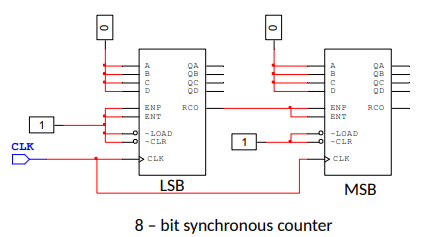
\includegraphics[width=10cm]{4bitsyncCascaded.png}

        \subsection{Truncated MOD}
            *What if you don't want to use the full MOD of a synchronous counter? (and don't want to create a custom one with state diagrams)
            \begin{itemize}
                \item use the load and initial count inputs ot specify the MOD of a counter
                \item For example, a MOD 16 4 bit counter can be configured into a MOD 4 counter.
                \item *Use the RCO output ot reload the inital count value
            \end{itemize}

        \subsection{Frequency Divider}
            Any counter will divide the input clock on the output of the fip flops. Thus, the output of a counter can be used as a clock elsewhere in a digital system.
            
            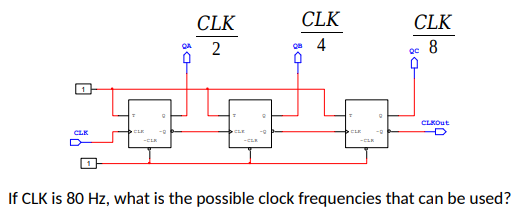
\includegraphics[width=12cm]{Freqdiv1.png}
            The MOD value is the value a counter can divide frequency of a clock.
            \begin{itemize}
                \item 1KHz clock put into a 25 MOD counter \ra~counter will divide the clock by 25 For every 25 pulses on the clock, 1 pulse is generated
            \end{itemize}
        
            \subsubsection{Potential Problems}
            *The output of the RCO (sync.) or the NAND gate (async.) to reset the counter is typically very small in width*
            \begin{itemize}
                \item Can create problems in using these for a clock signal on another circuit
                \item clock must have equal time high and low
            \end{itemize}
            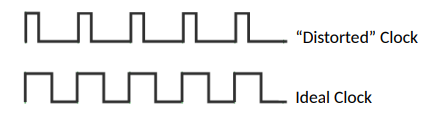
\includegraphics[width=13cm]{distortedVidealCLK.png}
            \\using a T flip flop will make the output equal HIGH and LOW time
            \begin{itemize}
                \item Placing through a fliop flop further divides frquenc by 2
            \end{itemize}
            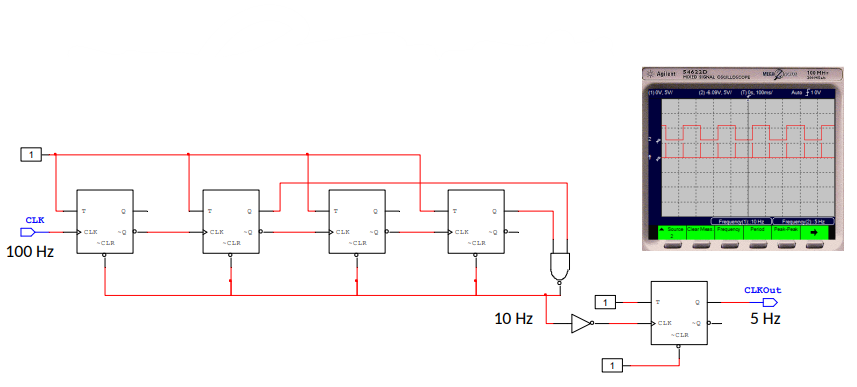
\includegraphics[width=15cm]{creatingClockSig.png}
            \\below is an example of a synchronous clock\\
            \includegraphics*[width=12cm]{SyncExample.png}
\end{document}